\documentclass{scrartcl}
\usepackage[utf8]{inputenc}
\usepackage[T1]{fontenc}

\usepackage[american]{babel}
\usepackage[autostyle, english = american]{csquotes}
 \usepackage[maxbibnames=10,
   backend=biber]{biblatex}
 \addbibresource{../bibliography.bib}

\usepackage[final,tracking=smallcaps,expansion=alltext, protrusion=true]{microtype}
\SetTracking{encoding=*, shape=sc}{50} %latex & friends, page 52
\usepackage{todonotes}
\usepackage{caption}
\usepackage{booktabs}
\usepackage{siunitx}
\usepackage{etoolbox}

\newrobustcmd*{\bftabnum}{%
  \bfseries
  \sisetup{output-decimal-marker={\textmd{.}}}%
}
\sisetup{detect-weight=true,detect-inline-weight=math}


\usepackage{float}
\usepackage{subcaption}
\usepackage{bm}
\usepackage{amsmath}
\usepackage{amsfonts}
\usepackage{amssymb}
\usepackage{nicefrac}
\usepackage{mathtools} % for \mathclap
\usepackage{hyperref}
\usepackage[noabbrev]{cleveref}
\usepackage{placeins}
\newcommand{\creflastconjunction}{, and\nobreakspace} % use Oxford comma
%\usepackage{placeins} % for floatbarrier

\usepackage{tikz}
\usetikzlibrary{arrows, positioning, shapes.geometric}
\usetikzlibrary{calc}
\graphicspath{{../../figures/}}

\newcommand{\img}{\bm{f}} % TODO: Format

\begin{document}
\title{Deep-Learning-based Image Denoising in Ophthalmology}
\author{Lukas Krenz}

\maketitle

\section{Introduction}
Intraoperative medical imaging is an important part of modern urgery.
During ophthalmic procedures, the surgeon manipulates anatomical structures of the retina with micron-scale maneuvers while observing the scene indirectly via microscope.
The resulting magnification has the effect that only a small area is focussed, other parts are either distorted or occluded.
Additionally, the motion of the eye introduces blur.
All these factors result in images which are corrupted by noise.
This makes precise operations more difficult.
Intraoperative images not only differ from the diagnostic ones in terms of quality.
During surgery, instruments are present and the membrane is stained with a coloring agent to amplify its edges.

Our goal is to increase the resolution of retinal fundus images both for diagnostic and intraoperative images.
Assuming that we have an image that was downsampled by an unknown operator, the goal is to find the best reconstruction of the original image.
We consider two different models:
\begin{itemize}
\item Downsampling by decresead spatial resolution.
  In our case we want to reconstruct an image that was downscaled by a factor of $2$ or $4$.
  This problem is called single image super resolution.
\item Downsampling by decreased sharpness.
  For this case we try to increase the quality of images by removing blur.
\end{itemize}

An image restoration algorithm has to fulfil the following requirements to be considered useful in an intraoperative setting:
\begin{enumerate}
\item All processing should happen in real time.
\item It has to work with images of varying quality, level of zoom and different positions of surgical instruments.
\item The anatomical structure, the position of surgical instruments, and the color have to be conserved.
Both blood vessels and the border of the membrane should be at least as clearly visible as in the original images.
This implies that we have to preserve the image edges.
\end{enumerate}
These constraints can be fulfilled by a deep learning approach.

We make the following contributions:
\begin{itemize}
\item We compare different loss functions, including adversarial training, and their suitability for the restoration of fundus images.
\item We present deep-learning models that are able to reconstruct images detoriated by both mentioned downsampling operators in in real-time for small crop sizes.
\item We evaluate the resulting algorithms with multiple metrics and discuss the consequences for intraoperative applications.
\end{itemize}

\section{Architectures}
\begin{figure}[ht]
  \centering
  \begin{subfigure}[b]{0.49\textwidth}
  \includegraphics[width=1.0\textwidth]{{nn_lapsrn}}
  \caption{LapSRN~\cite{LapSRN}}
  \label{fig:lapsrn}
  \end{subfigure}\quad\begin{subfigure}[b]{0.48\textwidth}
  \includegraphics[width=1\textwidth]{{nn_lapdeblur}}
  \caption{LapDeblur}
  \label{fig:lapdeblur}
  \end{subfigure}
  \caption{Generator architectures inspired by~\cite{LapSRN}.
    Blue and gray images show input and output images respectively.
    The symbol ($\bm{\ast}$) marks convolutions, ($\bm{\uparrow}$) resize-convolutions and 
    ($\bm{+}$) corresponds to element-wise addition
    All convolutions have 64 filters of size 3 with a padding and stride of 1.
    All convolutions except the ones in the resize-convolutions in the image reconstruction branch are followed by a leaky rectified linear unit with a negative slope of $0.2$.
    \label{fig:networks}
  }
\end{figure}
We use a modified \textbf{LapSRN} architecture (\cref{fig:lapsrn})~\cite{LapSRN}.
The network utilises a Laplacian pyramid, it first performs 2x upscaling and then 4x upscaling.

This architecture consists of two branches.
The first is the \textit{image reconstruction branch} and upscales the low resolution image using simple upscaling filters.
The second branch extracts features from the low resolution image using stacked convolutions and predicts the residual for each upscaled image of the first branch.
We use a depth of 10 per output resolution for this \textit{feature extration branch}.

Our model differs in three ways from the original architecture:
\begin{itemize}
\item We use three-channel \textsc{rgb} images both as input and output instead of working only on the Y-channel.
\item Instead of transposed convolutions we use resize-convolution blocks.
  They are composed of a nearest neighbour interpolation, a reflect-pad of size one and a standard convolution.
  They lead to fewer checkerboard artefacts than transposed convolutions, especially when they are used with adversarial learning~\cite{deconvolution}.
\item We only consider 4x upscaling here, but the approach can be easily extended to larger upscaling ratios.
\end{itemize}

For the deblurring case, we modify the architecture (\cref{fig:lapdeblur}) by removing the upsampling blocks from the \textit{feature extraction branch}.
Additionally, instead of using a \textit{image reconstruction branch}, we compute the residuals for input images directly.
Because all convolutions now operate in high-resolution space, we use 5 convolutions per output.
This approach has the advantage that we can use similar models for both downsampling operators.

We use the \textbf{PatchGan}~\cite{PatchGAN} discriminator for adversarial learning.
This is a fully convolutional network that penalizes on a basis of $70\times70$ patches.
In contrast to~\cite{PatchGAN} we use instance normalization~\cite{InstanceNorm} instead of batch normalisation layers.
Its architecture can be seen in \cref{fig:patchd}.

\begin{figure}[htb]
  \centering
  \includegraphics[width=0.5\textwidth]{{nn_patchd}}
  \caption{
Discriminator architecture from~\cite{PatchGAN}.
The symbol ($\vert \cdots \vert$) indicates instance normalization,
($ \bm{\downarrow} $) and ($ \bm{\ast} $) are convolutions with stride 2 and 1 respectively
All convolutions have kernel size 4 and a padding of 1 and are followed by a leaky rectified linear unit with a negative slope of $0.2$.
The layers have an output size of 64, 128, 256, 512 and 1.
\label{fig:patchd}
  }
\end{figure}

\section{Loss functions}
An appropiate choice of loss function is important to achieve good reconstructions.
In this work we combine three loss functions:
A saliency weighted $L_1$-loss ensures the faithful reconstruction of important areas, a perceptual loss optimizes visual similarity and an adversarial loss reconstructs high-frequency image components.
This ensemble of loss functions is inspired by~\cite{SaliencyGAN} and is optimized for the reconstruction of retinal images.

\begin{figure}[htb]
\centering
\begin{subfigure}{0.25\textwidth}
\centering
    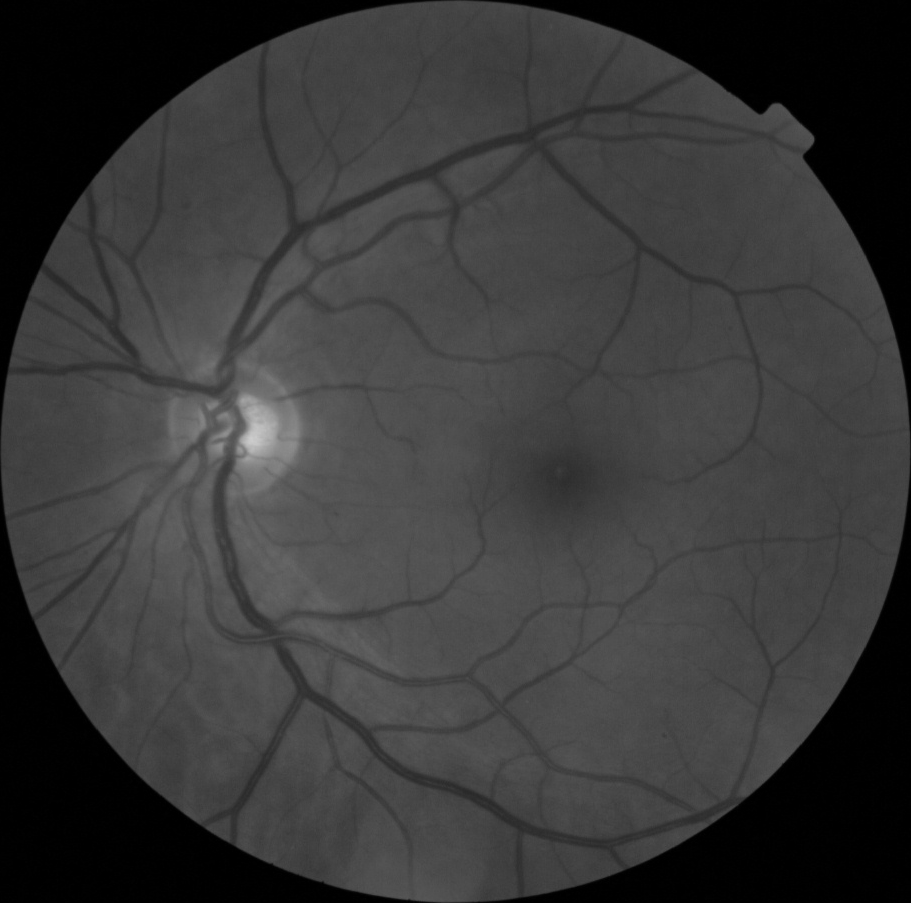
\includegraphics[width=1\textwidth]{saliency_gt}
    \caption{Input, Grayscale}
\end{subfigure}~
\begin{subfigure}{0.25\textwidth}
\centering
    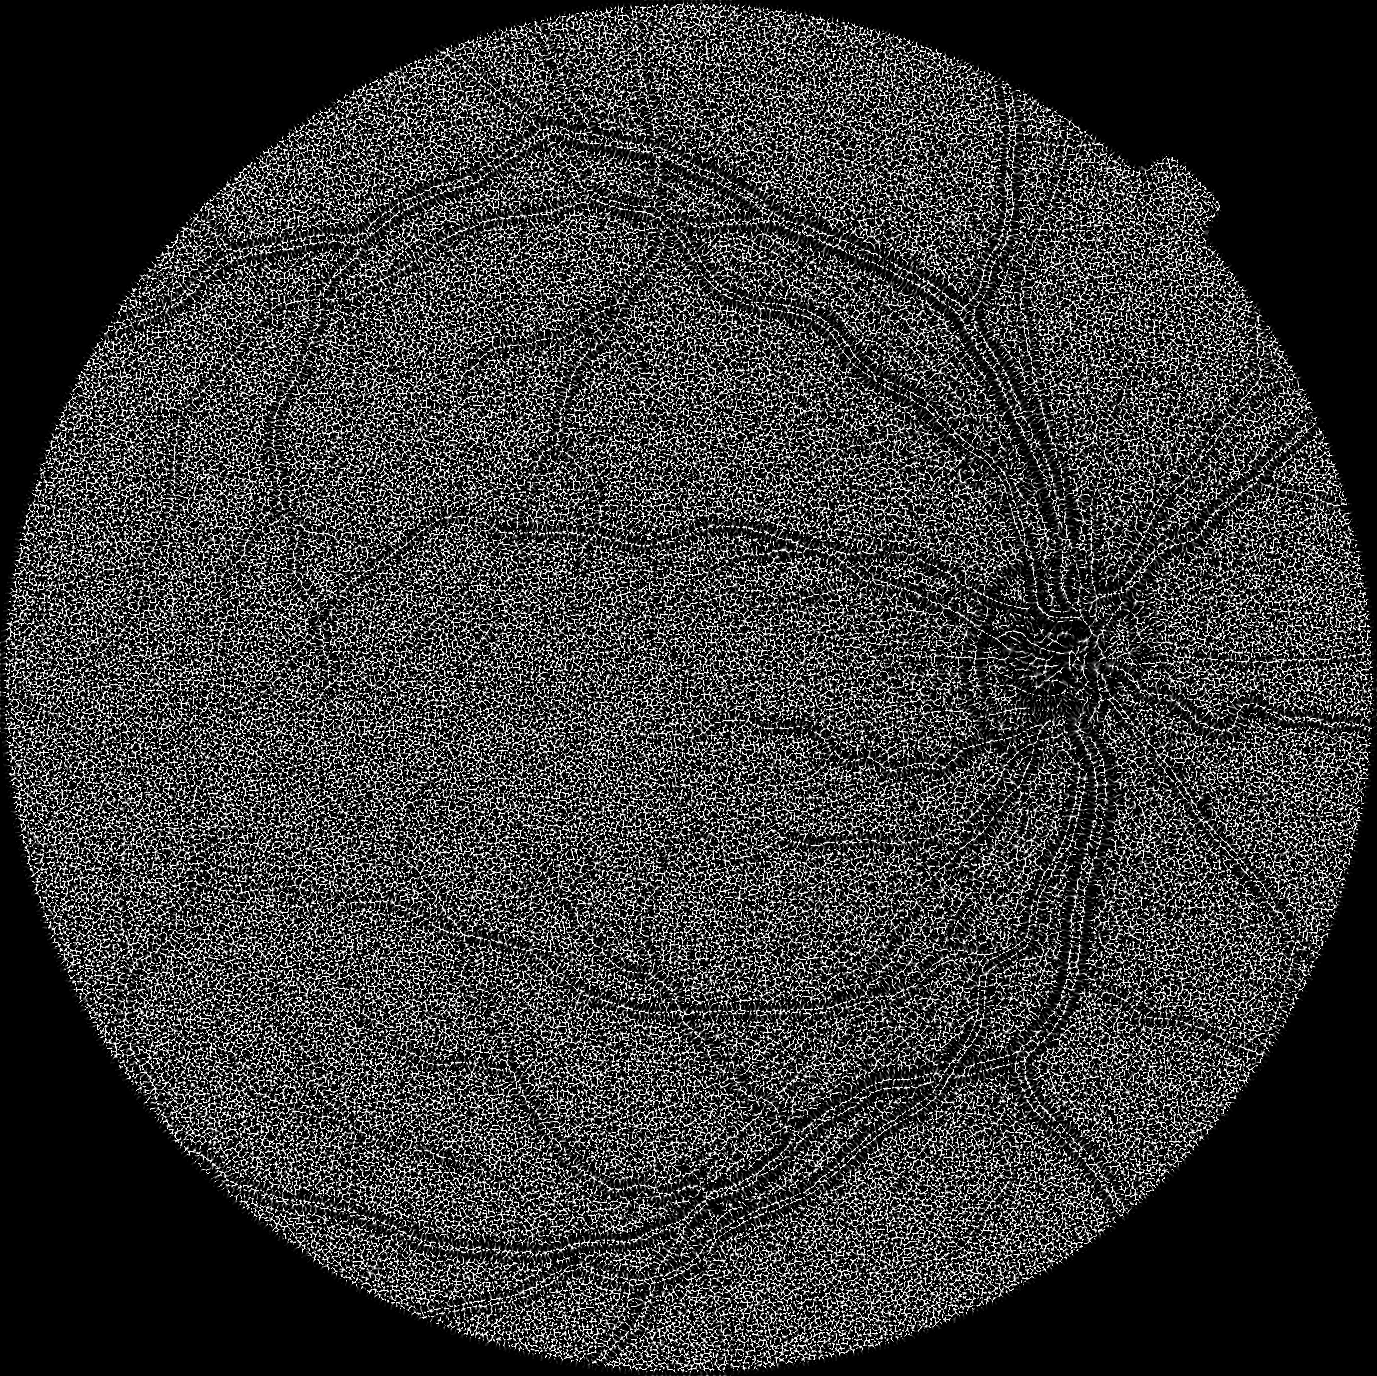
\includegraphics[width=1\textwidth]{saliency_vessels}
    \caption{$I_c$}
\end{subfigure}~
\begin{subfigure}{0.25\textwidth}
\centering
    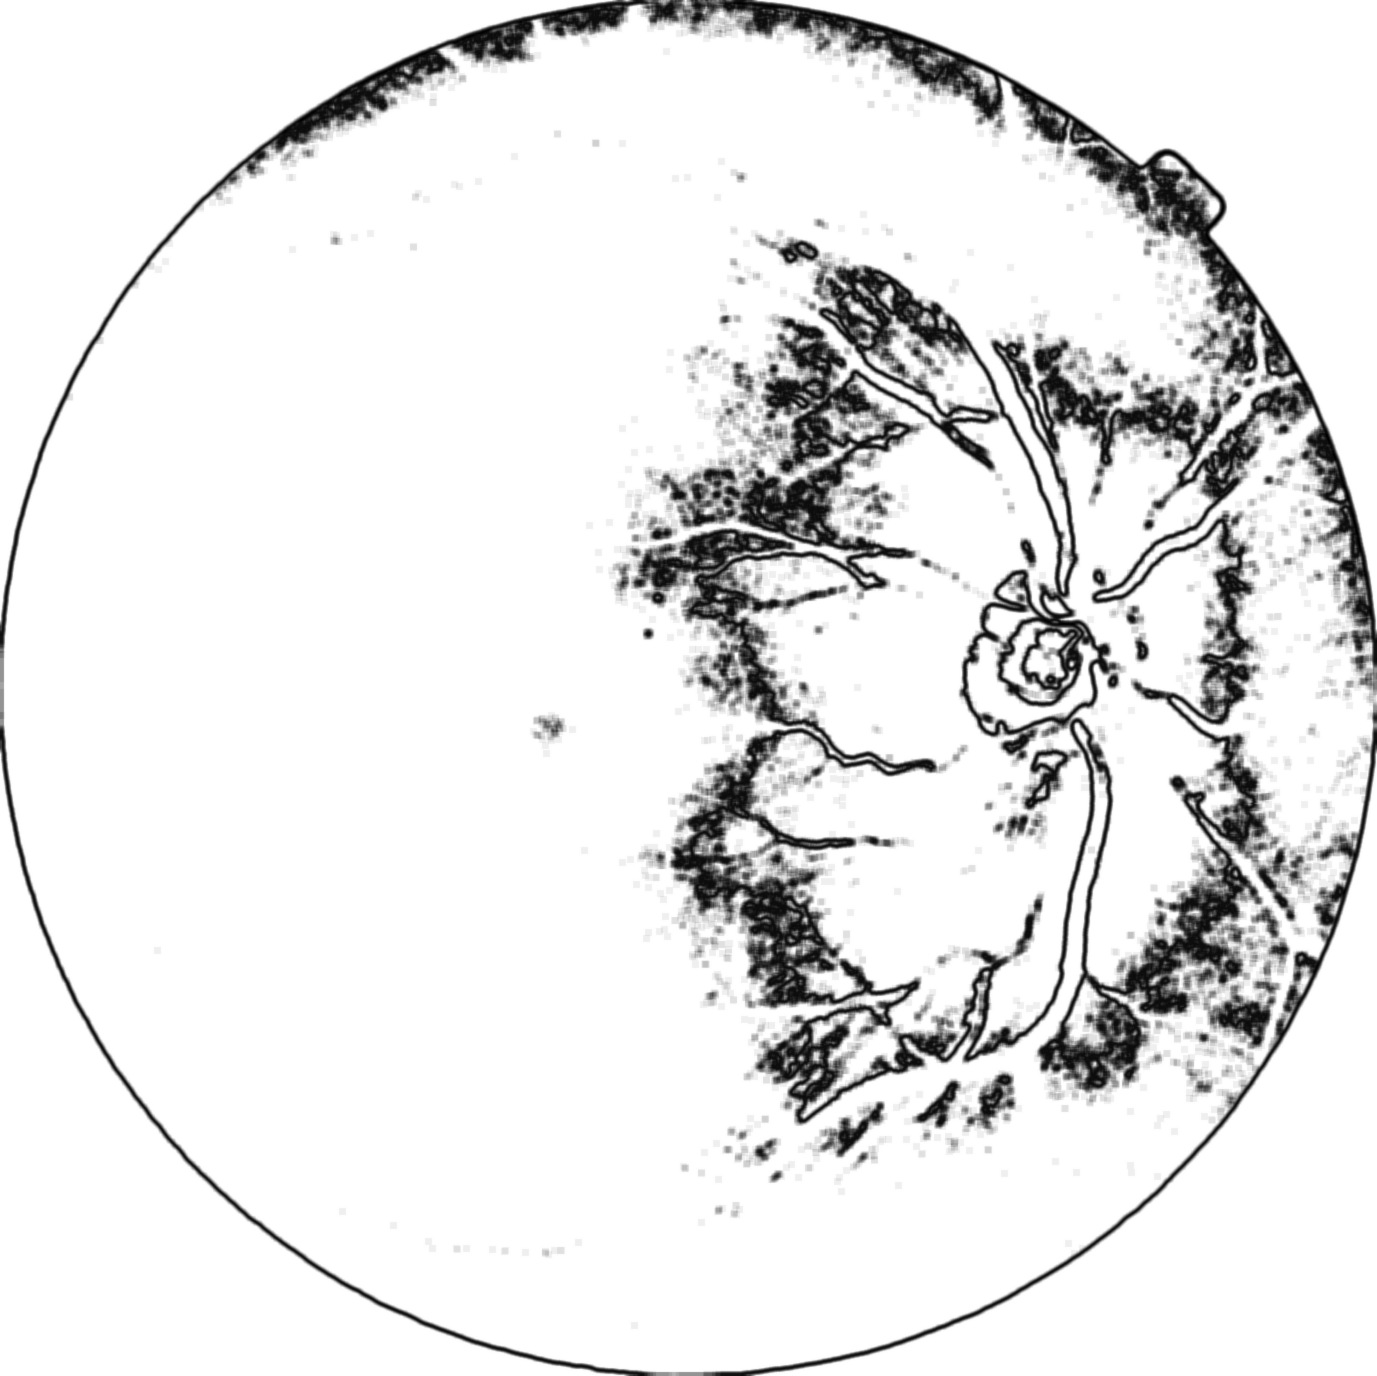
\includegraphics[width=1\textwidth]{saliency_entropy}
    \caption{$1 - I_e$}
\end{subfigure}~
\begin{subfigure}{0.25\textwidth}
\centering
    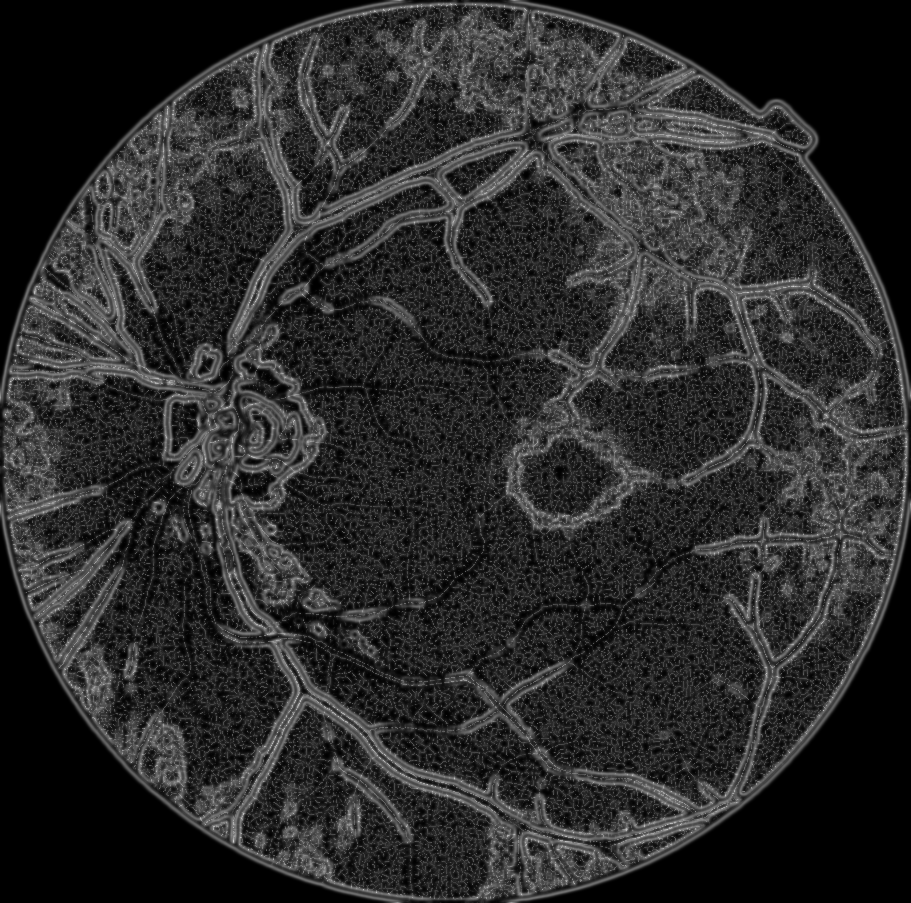
\includegraphics[width=1\textwidth]{saliency_full}
    \caption{$I_{\text{sal}}$}
\end{subfigure}

\caption{Components of a saliency map.
Brighter pixels indicate a higher weight.}
\label{fig:saliency}
\end{figure}

While the images in standard super-resolution tasks do not share a lot of common structure, retinal fundus images are visually similar to each other.
This can be used to create hand-crafted saliency maps that highlight relevant pixels.
We use maps that are similar to the ones of~\cite{SaliencyGAN}.
These saliency map consists of two components: curvature and local entropy.
The map and its components are shown in \cref{fig:saliency}.

The curvature map highlights fine structure in the image and can be computed as
\begin{equation}
 I_c = \frac{\img_{xx} \img_y^2 + \img_{yy} \img_x^2 - 2 \img_{x} \img_{xy} \img_{y} }{(\img_x^2 + \img_y^2)^{1.5}},
\end{equation}
where \(\img\) is the intensity of the image and subscripts represents its derivatives~\cite{SaliencyGAN}.
We approximate the image derivatives by convolving the image with derivatives of Gaussians with \(\sigma = 1\).
Undefined elements of the feature map are defined to have a weight of zero.
We clip the resulting feature map to the range of $[0,1]$.

The local entropy map highlights pixels that are in a neighborhood that contain more information.
We compute the entropy for each pixel by
\begin{equation}
  \label{eq:entr}
  I_e = - \sum_{s \in P_s} p(s_i) \log(p(s_i)),
\end{equation}
where \(p\) is the probability that a pixel \(s\) has an intensity of \(s_i\) in a patch \(P_s\).
The probability $p(s_i)$ is estimated by a normalised histogram with eight bins of equal size, computed for each patch seperately.
A patch is composed of the pixel itself and its surrounding neighborhood of size \(7 \times 7\).
We then convolve the image with a Gaussian filter with \(\sigma = 0.5\) to remove high-frequency noise.
Finally we normalize $I_e$ to the range \([0, 1]\) and use $1 - I_e$ for our saliency map.
This highlights compact regions of the image.

We then compute the uniqueness of each pixel of a feature map \(f\) with the function
\begin{equation}
  \label{eq:uniq}
  U(m) = \sum_{o \in P_c} w(c, o) \vert m(c) - m(o) \vert,
\end{equation}
where \(c\) corresponds to the pixel in the middle of a patch \(P_c\) of size \(7 \times 7\).
The function \(w(a,b) = \exp(d(a, b))\) weights the pixels by their Euclidean distance \(d\).
All uniqueness maps are normalized to the range \([0,1]\).

Finally, we combine the uniqueness maps of both components linearly
\begin{equation}
  \label{eq:saliency}
  I_{\text{sal}} = 0.4 \cdot U(I_c) + 0.6 \cdot U(1 - I_e)
\end{equation}
to obtain the saliency map for each image~\cite{SaliencyGAN}.

We then use this map to weigh the pixel-wise error.
We propose a weighted version of the Charbonnier loss.
It is a differentiable approximation of the $L_1$ loss which leads to sharper edges compared to a standard \textsc{mse}-loss~\cite{LapSRN}.
Our weighted loss can be described by
\begin{align}
\label{eq:charbonnier}
  L_{\text{sal}}( \hat{\bm{\img}}, \bm{\img}) = \Vert I_{\text{sal}}(\img) \circ \sqrt{ (\hat{\img} - \img)^2 + \varepsilon} \Vert_1,
\end{align}
where $\varepsilon$ is a parameter set empirically to $1e-6$ for our experiments and \(\circ\) denotes the element-wise product.

Secondly, we use a perceptual loss~\cite{PerceptualLoss}.
It does not compare images pixel-wise but consideres the difference of filtered images.
We use the feature activations of the first and second pooling layer of a VGG-16 network~\cite{Vgg} trained on Imagenet.
The resulting loss is
\begin{equation}
  \label{eq:perceptual-loss}
  L_p(\img, \hat{\img}) = \sum_{\mathclap{l \in \{ \text{pool}_1, \text{pool}_2 \}}} \Vert \phi_l( \hat{\img} ) - \phi_l (\img) \Vert_2^2,
\end{equation}
where \(\phi_l\) denotes the activations of the layer \(l\).
This leads to perceptually better images but decreased PSNR.
See~\cite{PerceptualLoss} for motivation and details.

We use an adversarial loss as our final building block, similar to~\cite{SRGAN}.
Training then resembles a two-player game between a generator \(G\) an a discriminator \(D\).
The discriminator tries to decide, whether an image is a ground-truth high-resolution image or an low resolution image that was upsampled by the generator.
The generator is trained to fool the discriminator.
Both networks are trained alternatingly.
This is realized as the optimization problem~\cite{GAN}
\begin{align}
 \min_G \max_D \mathbb{E}_{\bm{x} \sim P_r} \left[ \log (D({\bm{x}})) \right] +
  \mathbb{E}_{\hat{\bm{x}} \sim P_g} \left[  \log (1 - D(\hat{\bm{x}})) \right].
\end{align}
To improve stability, the generator minimizes
\begin{equation}
  L_a = - \mathbb{E}_{\hat{\bm{x}} \sim P_g} \left[ \log (D(\hat{\bm{x}})) \right]
\end{equation}
instead.
The patch-discriminator does not predict a single probablity per image but rather one per image patch.
Thus, the probability distributions $P_r$ and $P_g$ correspond to the distribution of real high-resolution patches and super-resolved patches respectively.
This discriminator design is able to discover high-frequency image details while relying on the other two losses for low-frequency content~\cite{PatchGAN}.
Note that we only penalize the last output image by the adversarial loss.

The total loss function is then
\begin{equation}
  \label{eq:total-loss}
L_\text{total}(\hat{\img}, \img) = \frac{1}{3 W_{\img} H_{\img}}
\left( \sum_{\img, \hat{\img}}
  5 L_{\text{sal}} (\hat{\img}, \img) + 0.12  L_p(\hat{\img}, \img) \right) + 0.01 L_a,
\end{equation}
where the sum runs over all model outputs \(\hat{\img}\) and the corresponding ground truth \(\img\).
All losses are normalised by number of channels (3), image height \(H_{\img}\) and width \(W_{\img}\).
The weights for saliency and perceptual loss are chosen such that they are of similar size, the adversarial weight was chosen empirically.

\section{Implementation \textit{\&} Training Details}
We use the Messidor dataset~\cite{Messidor} which consists of 1200 high resolution fundus images.
The black borders from the images were removed.
We used 80\% of the dataset for training, the rest was used for validation.
The high resolution images are augmented by:
\begin{itemize}
\item A random scaling with a factor uniformly distributed between $0.5$ and $1.0$.
  We rescale using bicubic downsampling.
\item Random crop of size $128 \times 128$ chosen by rejection sampling:
If a crop contains more than $50\%$ black pixels (gray-scale value smaller than 90) or no vessels it is rejected and another crop is chosen.
The vessels are detected using a pre-computed Frangi filter~\cite{Frangi}.
We consider a crop to contain no vessels when fewer than $64$ pixels are marked as vessels by the Frangi filter.
This threshold was chosen empirically.
\item Random rotation by either $0, 90, 180, \text{or } 270$ degrees.
  These roations do not change the size of the image and thus need no rescaling.
\item Random vertical and horicontal flip, each with a probability of $50\%$.
\item Specular reflections with a probability of $25\%$.
This is simulated by increasing the intensity of the image in a circular mask (post-processed with a Gaussian filter) by a random intensity.
The specular reflection mirror the usage of light sources during operations.
\end{itemize}
Note that all augmentations (except specular reflections) are also applied to the pre-computed saliency-maps and the random scaling is applied on the vessel segmentations.
The scaling, rotation and flipping augmentations are also used by~\cite{LapSRN}.

We obtain low resolution images by a Gaussian blur with maximum radius of three for denoising
For the super-resolution network, we first apply a gaussian blur with a maximum radius of two and then use bicubic downsampling with factors 2 and 4.
The blurring is done by first selecting a random total blur radius, sampled uniformally between zero and the maximum blur.
We then distribute the blur such that the intermediate image is blurred with half strength.
This intermediate blur can be computed by \( \left( \text{radius}_{\text{total}} / \sqrt{2} \right)\), using the fact that a convolution of two Gaussians is a Gaussian.

Finally, images and saliency maps are converted to tensors of range $(0,1)$.
Images are scaled by subtracting
\(
\begin{bmatrix}
 0.485 & 0.456 & 0.406 
\end{bmatrix}
\)
and dividing by
\(
\begin{bmatrix}
0.229 & 0.224& 0.225
\end{bmatrix}
\).
This is the normalisation that is expected from the pre-trained VGG-16 network.

We use a batch size of $64$ for all experiments.
An epoch thus consists of $15$ gradient updates.

All weights of the generator are initialised with Xavier initialisation~\cite{Xavier}, all weights of the discriminator are drawn from a normal distribution with mean zero and variance of 0.02~\cite{PatchGAN}. 
We first train solely the generator without adversarial loss.
It is optimized by \textsc{adam}~\cite{Adam} with an initial learning rate of $10^{-4}$ for the super-resolution network and $10^{-5}$ for the deblurring network.
We use a weight decay of $10^{-5}$.
The super-resolution generator is trained for $9999$ epochs, the deblurring generator for $6666$ epochs.
The learning rate is divided by ten every $3333$ epochs.

The resulting network is then used to initialise the adversarial training, which is trained for another $6666$ epochs.
We use the same learning rate for both networks, starting with an initial value of $10^{-5}$, using the same learning rate schedule as for the initial training.
Both networks are optimised by \textsc{adam} with the momentum term $\beta_1$ set to $0.5$ for improved stability~\cite{Dcgan}.
No weight decay is used in this stage.

The network is implemented was Pytorch~\cite{Pytorch} and was trained using a Titan X.
Training takes \SI{20}{\hour} for the super-resolution network without adversarial loss and an additional \SI{29}{\hour} for the adversarial training.
The deblurring network took \SI{34}{\hour} for the initial training and an additional \SI{48}{\hour} for adversarial training.

\section{Evaluation}
We use the \textsc{mse}-based metric \textsc{psnr} to compare images on a pixel-wise basis.
Additionally, we use the structural similarity(\textsc{ssim})~\cite{Ssim} which uses a model based on human perception.
Following standard procedure, we apply these metrics on gray-scale versions of our images.
For our chosen application, the correct reconstruction of image gradients is important, for example to enhance the border of the retina membrane.
To do this, we compute the gradient magnitude with a Sobel filter and compare the reconstruction.

Similarly to~\cite{SaliencyGAN} we use vessel segmentation to evaluate the accurate reconstruction of image details.
For this we use two methods:
\begin{enumerate}
  \item The Frangi filter~\cite{Frangi} is a simple segmentation method.
  We use the implementation of~\cite{Scikit-image} with parameters $\beta_1 = 0.7, \beta_2=0.01$ with a scale range of $(0, 3)$.
  Pixels with a intensity of $0.2$ or large are marked as vessels.
  These parameters were found with a grid search on the training set.
  The method is not robust, sometimes a blurry images leads to a more accurate reconstruction.
  This is why compare the reconstruction of the Frangi segmentation instead of the segmentation accuracy.
\item As an example for a state-of-the art deep-learning based algorithm we use~\cite{RetinaUnet}.
  It is based on the \textbf{UNet}-architecture~\cite{Unet}.
  For this method we report the area under the \textsc{ROC}-curve (\textsc{AUC}).
\end{enumerate}
We evaluate this on the testing set of the DRIVE dataset~\cite{Drive}, for which a ground truth segmentation is available.
We compare the super resolution network with bicubic interpolation.
Images are first reflect padded to have a size divisable by 4 for SR and 16 for deblurring.
This padding is then removed before all comparisons.
We cut off an additional stripe of size equal to the upsampling factor for the super-resolution network.
\begin{table}[htb]
\centering
\caption{Results for super resolution models on our validation dataset (Messidor~\cite{Messidor}) for both possible upsizing factors.
  The full model is not compared for the $2\times$ model because the adversarial loss is only applied to the largest output image.
  Best results are bold.
}

\label{tab:results-sr-messidor}
\begin{tabular}{@{}llS[table-format=2.2]S[table-format=2.3]S[table-format=2.2]@{}}
\toprule
{Model} & {Factor} & {PSNR} & {SSIM} & {Sobel \textsc{mse} \SI{1e4}{}}\\ \midrule
Bicubic & 2 & 44.67 & 0.972 & 2.56 \\
Perceptual & 2 & 42.21 & 0.945 & 1.25 \\
Saliency & 2 & \bftabnum 45.30 &  \bftabnum 0.973 & 1.33 \\
Saliency + Perceptual & 2 & 44.83 & 0.969 & \bftabnum 1.22 \\ \midrule

Bicubic & 4 & 40.69 &  0.951 & 8.35 \\
Perceptual & 4 & 42.22 & 0.943 & 2.53 \\
Saliency & 4 & \bftabnum 42.82 & \bftabnum 0.953 & 3.59 \\
Saliency + Perceptual & 4 & 42.23 & 0.945 & \bftabnum 2.51 \\
Full & 4 & 41.78 & 0.942 & 2.64 \\
\bottomrule
\end{tabular}
\end{table}%
To evaluate the effectiveness of our chosen loss function, we trained different combinations with the same training schedule.
We first evaluated on our hold-out validation dataset (\cref{tab:results-sr-messidor}).
For an example image patch for this dataset, see \cref{fig:messidor-example}.
Secondly, we evaluated on the Drive~\cite{Drive} dataset (\cref{tab:results-sr-drive}). 
An example segmentation for all loss function is shown in \cref{fig:segmentation-example}.
\begin{description}
\item[Saliency] The saliency weighted $L_1$-loss leads to an accurate, albeit blurry, reconstruction of important features of the fundus.
  It results in the highest \textsc{psnr} and \textsc{ssim}.
  Some textural details are missing and edges of vessels are not clear.
  It has the worst segmentation results, tiny details are lost for this reconstruction.
\item[Perceptual] The perceptual loss results in lower \textsc{psnr} and \textsc{psnr} but the images are more realistic and visually more pleasing.
  It introduces regular artifacts and leads to the best reconstruction of the Frangi segmentation.
  This loss achieves a \textbf{UNet} segmentation result that is nearly as good as the loss ensemble, indicating that it is the most important component.
\item[Saliency \textit{\&} Perceptual] Combining both losses results in a reconstruction that is a good compromise between faithful pixel-wise reconstruction and perceptual quality.
  The artefacts are still visible but with a smaller intensity.
  It has the lowest Sobel-\textsc{mse} which indicates that it is able to restore image gradients more correctly.
  Additionally, it restores the Frangi segmentation as correctly as the perceptual loss alone and has the second best \textbf{UNet} segmentation.
\item[Saliency \textit{\&} Perceptual \textit{\&} Adversarial]
  The addition of the adversarial loss improves the reconstruction of texture, the images are sharper.
  Additionally, it removes the artefacts introduced by the perceptual loss.
  It leads to the best \textsc{auc} for the \textbf{UNet} segmentation.
  The downside of this loss is that it the adversarial component is not trained to reconstruct the image correctly.
  This can lead to additional failure cases where the network hallucinates details, such as additional blood vessels.
\end{description}
Overall, our loss ensemble results in both correct reconstruction and visually convincing results.
This is true as well for the $2 \times$ scaled output.
The adversarial loss trades faithful reconstruction for sharper images.
With and without it, our proposed loss combination achieves competitive results on both datasets.

\begin{table}[t]
\centering
\caption{Results for super resolution models on the Drive~\cite{Drive} (testing) dataset.
  AUC corresponds to area under the \textsc{roc} curve achieved by running the retina-unet~\cite{RetinaUnet} on the upscaled images.
  Best results are bold.
}

\label{tab:results-sr-drive}
\begin{tabular}{@{}lS[table-format=2.2]S[table-format=2.2]S[table-format=2.2]S[table-format=2.3]S[table-format=2.3]@{}}
\toprule
{Model} & {PSNR} & {SSIM} & {Sobel \textsc{mse} \SI{1e4}{}} & {Frangi Reconstruction Acc.} & {AUC UNet} \\ \midrule
Ground Truth & $\infty$ & 1.00 & 0.00 & 1.00 & 0.979 \\
Bicubic & 35.27 & 0.92 & 29.87 & 97.05 & 0.852 \\
Perceptual & 38.90 & 0.93 & 8.61 & \bftabnum 98.62 & 0.943 \\
Saliency & \bftabnum 39.50 & \bftabnum 0.94 & 8.55 & 98.35 & 0.921 \\
Saliency + Perceptual & 39.20 & 0.93 &\bftabnum 7.84 & \bftabnum 98.62 & 0.946 \\
Full & 38.85 & 0.93 & 8.29 & 98.51 & \bftabnum 0.948 \\
\bottomrule
\end{tabular}
\end{table}

\begin{figure}[t]
\centering
\makebox[\linewidth][c]{%
\begin{subfigure}{0.2\textwidth}
\centering
    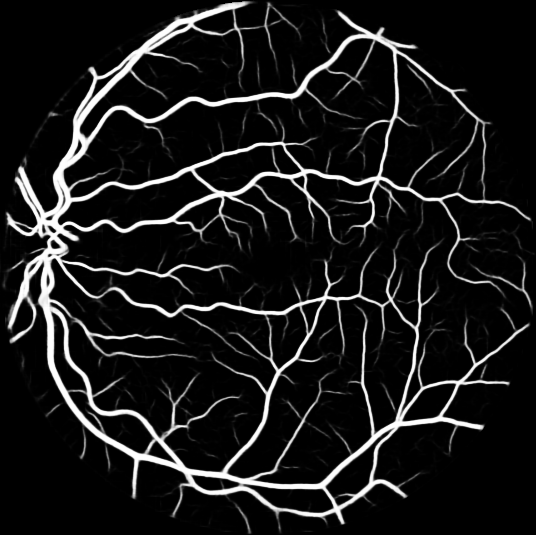
\includegraphics[width=1.0\textwidth]{segmentation_hr}
    \caption{HR}
\end{subfigure}~
\begin{subfigure}{0.2\textwidth}
\centering
    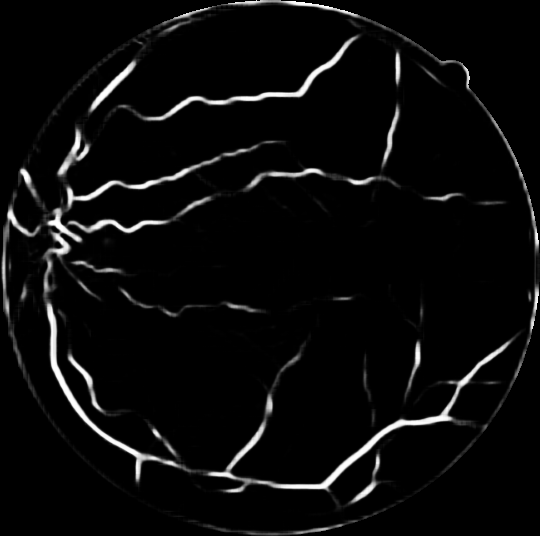
\includegraphics[width=1.0\textwidth]{segmentation_bic}
    \caption{Bicubic}
\end{subfigure}~
\begin{subfigure}{0.2\textwidth}
\centering
    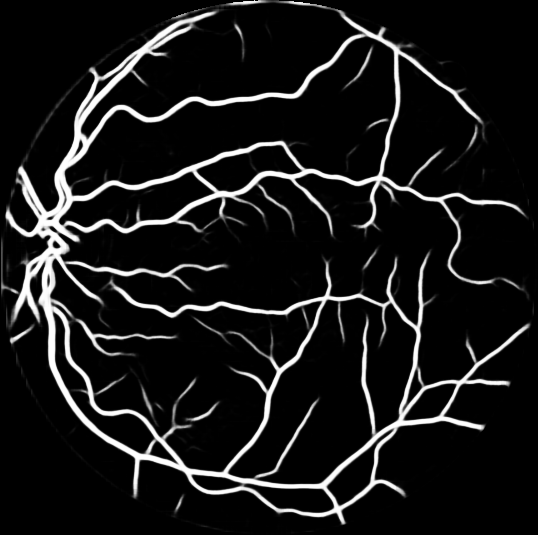
\includegraphics[width=1.0\textwidth]{segmentation_perc}
    \caption{Perceptual}
\end{subfigure}~
\begin{subfigure}{0.2\textwidth}
\centering
    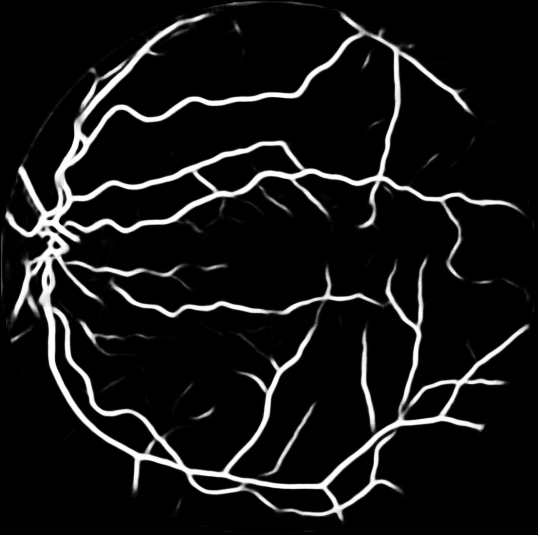
\includegraphics[width=1.0\textwidth]{segmentation_saly}
    \caption{Saliency}
\end{subfigure}~
\begin{subfigure}{0.2\textwidth}
\centering
    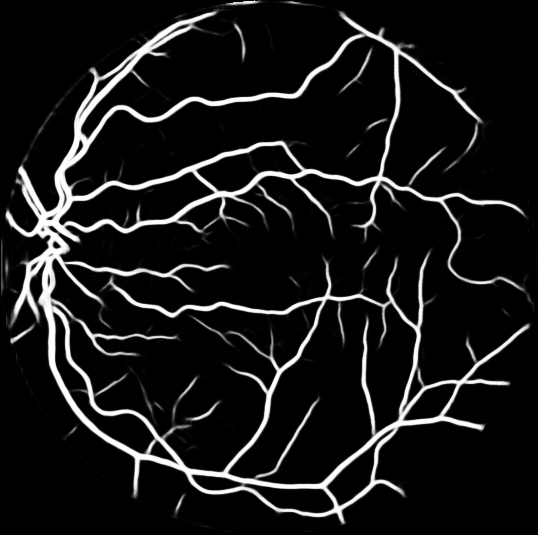
\includegraphics[width=1.0\textwidth]{segmentation_nogan}
    \caption{Sal.\ + Perc.}
\end{subfigure}~
\begin{subfigure}{0.2\textwidth}
\centering
    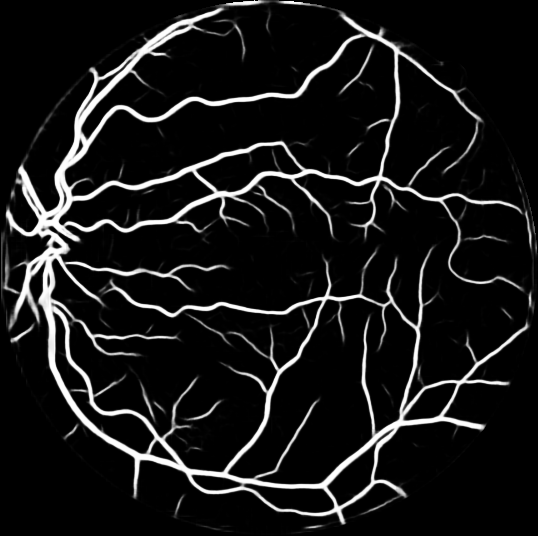
\includegraphics[width=1.0\textwidth]{segmentation_gan}
    \caption{Full Model}
\end{subfigure}
}
\caption{Segmentation results on Drive~\cite{Drive} testing set.}
\label{fig:segmentation-example}
\end{figure}

\begin{figure}[htb]
\centering
\makebox[\linewidth][c]{%
\begin{subfigure}{0.2\textwidth}
\centering
    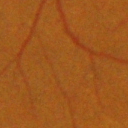
\includegraphics[width=1.0\textwidth]{patch_sr1_gt_small}
    \caption{HR}
\end{subfigure}~
\begin{subfigure}{0.2\textwidth}
\centering
    
\includegraphics[width=1.0\textwidth]{patch_sr1_bic_small}
    \caption{Bicubic}
\end{subfigure}~
\begin{subfigure}{0.2\textwidth}
\centering
    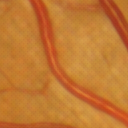
\includegraphics[width=1.0\textwidth]{patch_sr1_sal_perc_small}
    \caption{Perceptual}
\end{subfigure}~
\begin{subfigure}{0.2\textwidth}
\centering
    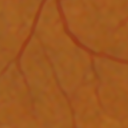
\includegraphics[width=1.0\textwidth]{patch_sr1_sal_small}
    \caption{Saliency}
\end{subfigure}~
\begin{subfigure}{0.2\textwidth}
\centering
    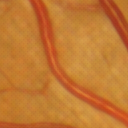
\includegraphics[width=1.0\textwidth]{patch_sr1_sal_perc_small}
    \caption{Sal.\ + Perc.}
\end{subfigure}~
\begin{subfigure}{0.2\textwidth}
\centering
    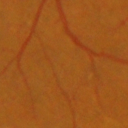
\includegraphics[width=1.0\textwidth]{patch_sr1_gan_small}
    \caption{Full Model}
\end{subfigure}
}
\caption{Upscaling results for an $128^2$ patch from our validation set (Messidor~\cite{Messidor})}
\label{fig:messidor-example}
\end{figure}

The deblurring network is compared to a standard \textbf{UNet} architecture~\cite{Unet} with \textsc{mse} loss, trained in the same manner as our network.
We use an implementation that does not crop feature maps for the skip connections but rather pads them such that they have the same shape.
This is a common architecure for bio-medical applications and similar architectures can be used successfully as generators for image-translation tasks~\cite{PatchGAN}.
Our network is able to improve the perceived image quality (\cref{fig:deblurring-example}), \textsc{ssim} and segmentation \textsc{auc} (see \cref{fig:deblurring-metrics}).
Note that the \textbf{UNet} achieves a better \textsc{ssim}-value but worse \textsc{auc}.

Even though we did not optimize our implementation for speed, super-resolving small image patches of size $128^2$ and deblurring patches of size $256^2$ is possible in real-time (\cref{fig:benchmark}).

A preliminary evaluation on intraoperative data did not show a significant improvement for both deblurring and super-resolution.
This could be caused by poor video quality.

\begin{figure}[htb]
\centering
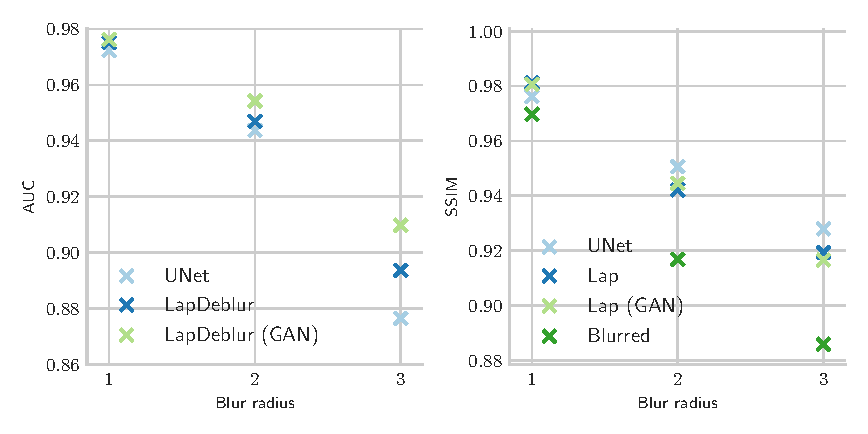
\includegraphics[]{deblur_complete_paper}
\caption{Performance metrics for deblurring on the Drive~\cite{Drive} dataset (testing).\\
Segmentation on blurred images directly leads to an AUC of 0.96, 0.83 and 0.65 respectively.}
\label{fig:deblurring-metrics}
\end{figure}

\begin{figure}[htb]
\centering
\begin{subfigure}{0.33\textwidth}
\centering
    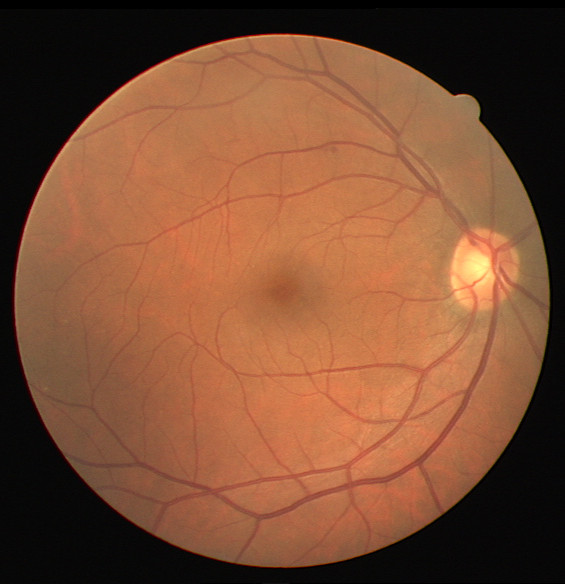
\includegraphics[width=1.0\textwidth]{deblur_gt}
    \caption{GT}
\end{subfigure}%
\begin{subfigure}{0.33\textwidth}
\centering
    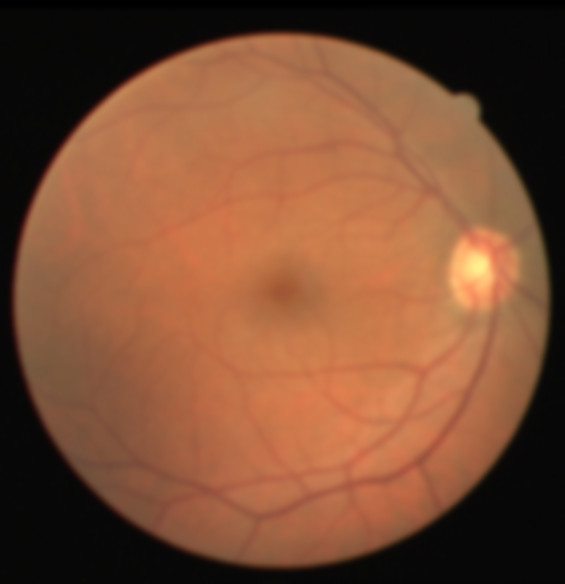
\includegraphics[width=1.0\textwidth]{deblur_lr}
    \caption{Blurred, Radius 3}
\end{subfigure}%
\begin{subfigure}{0.33\textwidth}
\centering
    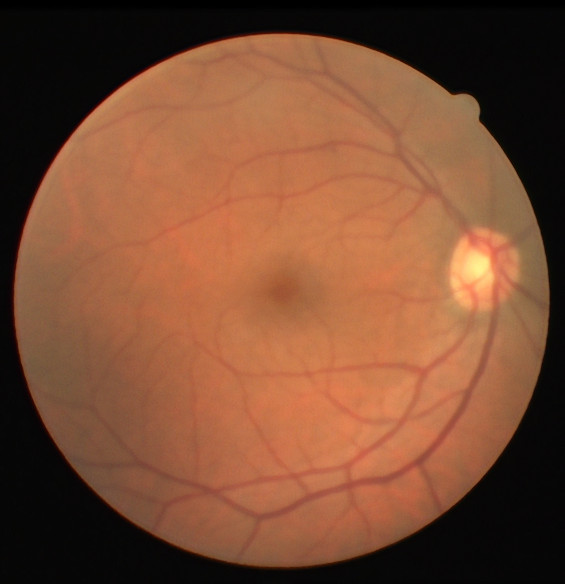
\includegraphics[width=1.0\textwidth]{deblur_gan}
    \caption{Deblurred with full model}
\end{subfigure}

\caption{Example for deblurring. Image from Drive (test)~\cite{Drive}}
\label{fig:deblurring-example}
\end{figure}


\begin{figure}[htb]
\centering
\begin{subfigure}{0.45\textwidth}
\centering
    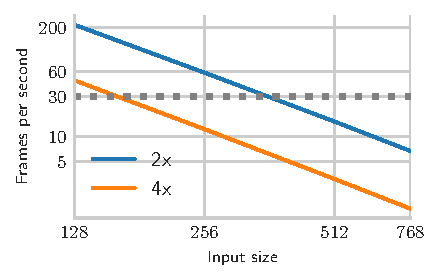
\includegraphics[]{time_upscaling_paper}
    \caption{Speed for upscaling}
\end{subfigure}\quad\qquad%
\begin{subfigure}{0.45\textwidth}
\centering
    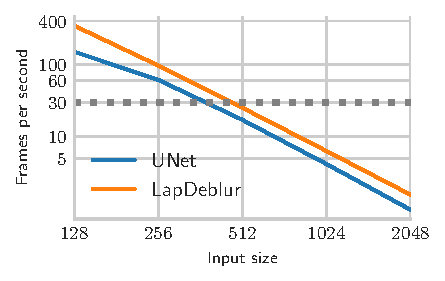
\includegraphics{time_denoising_paper}
    \caption{Speed for denoising}
\end{subfigure}
\caption{Frames per second vs.\ input image size.
Measured on a Titan X.}
\label{fig:benchmark}
\end{figure}

\section{Summary}
Our proposed models work well for diagnostic images.
They are efficient and result in both faithful and perceptual convincing images.
While the individual loss functions result in good reconstructions, our chosen ensemble is clearly superior by all used metrics.

The algorithms satisfy all our constraints for intraoperative usage:
\begin{itemize}
\item The algorithms work in real-time for small patch sizes without performance optimization.
  If a faster speed is desired our super-resolution network is also able to output $2\times$ resolved images.
\item The deblurring network is robust to different levels of blur.
  It is able to improve the segmentation results on all tested blur intensities.
  The super-resolution network is robust to blur due to the used data augmentations.
\item All networks except the ones trained with adversarial loss retain the structure of blood vessels.
  Our evaluation showed that the proposed loss ensemble recovers vessels, image gradients and overall detail better than all single loss functions.
  They retain the anatomical structure and other fine details.
\end{itemize}
We have thus shown that our proposed methods can be used successfully a pre-processor for other computer vision tasks or to provide a digital zoom.

\FloatBarrier
\printbibliography
\end{document}